\chapter{Experimental Evaluation}
\label{ch:experiments}

In this chapter we illustrate experimental studies that we have performed for the techniques described in \mychapter\ref{ch:profiling,ch:continuous}, which have been implemented in production systems and evaluated against prominent benchmarks.  

%typically evaluated against industry-strength benchmarks. For performance metrics, reported figures have been obtained by performing multiple runs in a Linux system with negligible background activity, and we also show confidence intervals stated at $95\%$ confidence level where possible.

In the first part of the chapter, we evaluate our space-efficient inter-procedural technique for context-sensitive profiling. In our analysis, we take into account a large collection of popular interactive Linux applications and industry-strength benchmarks. Results collected for a number of accuracy and space usage metrics reinforce the theoretical prediction that the HCCT achieves a similar precision as the CCT in a space that is several orders of magnitude smaller, and roughly proportional to the number of hot contexts. Our implementation is cast in a full-fledged infrastructure that we developed for profiling multi-threaded Linux C/C++ applications, and ships as a plugin for the GNU Compiler Collection. We also discuss how we integrated our technique with static bursting, resulting in faster running times without substantially affecting accuracy: we incur a slowdown competitive with the \gprof\ call-graph profiler while collecting finer-grained program profiles. 

In the second part, we discuss an implementation in the Jikes RVM of our intra-procedural technique for multi-iteration path profiling. We present a broad experimental study on a large suite of prominent Java benchmarks, showing that our profiler can collect profiles that would have been too costly to gather using previous multi-iteration techniques. The key to the efficiency of our approach is to replace costly hash table accesses, which are  required by the Ball-Larus algorithm to maintain path counters for larger programs, with substantially faster operations on trees. We then study structural properties of path profiles that span multiple iterations for several representative benchmarks, and discuss memory footprints of the \ksf\ and \kipf\ data structures for increasing values of $k$.

Finally, we present an extensive experimental evaluation of our OSR techniques for continuous program optimization. We first analyze the performance of \osrkit\ in the \tinyvm\ proof-of-concept virtual machine that we developed in LLVM. Our goal is to address a number of typical concerns of VM builders, measuring, e.g., the impact of having an OSR point in a hot code portion, and the actual cost of performing an OSR transition. We then present an LLVM implementation of the techniques for automatically constructing OSR mapping described in \mysection\ref{ss:osr-mapping-algorithms}, evaluating the fraction of program locations where they allow OSR to be efficiently fired in prominent benchmarks. Our experiments suggest that bidirectional OSR transitions between rather different program versions can be supported almost everywhere in the code under several classic optimizations.

\ifdefined \noauthorea
\section{HCCT Construction and Accuracy}

In this section, we present an extensive experimental study of our data streaming-based methodology for context-sensitive profiling. We implemented several variants of context-sensitive profilers and we analyzed their performance and the accuracy of the produced $(\phi,\varepsilon)$-HCCT with respect to a number of metrics and using many different parameter settings. Besides the exhaustive approach, where each routine call and return is instrumented, we integrate our solution with previous techniques aimed at reducing time overhead: we focus in particular on static bursting~\cite{Zhuang06}, which offers convenient time-accuracy tradeoffs. The experimental analysis not only confirms, but reinforces the theoretical prediction: the $(\phi,\varepsilon)$-HCCT represents the hot portions of the full CCT very well using only an extremely small percentage of the space required by the entire CCT: all the hottest calling contexts are always identified correctly, their counters are very accurate, and the number of false positives is rather small. With bursting, the running time overhead can be kept under control without affecting accuracy in a substantial way.

\subsection{Implementation}

\paragraph*{Compiler Plugin.} The \gcc\ compiler provides an instrumentation infrastructure to emit calls to analysis routines at the beginning and at the end of each function, passing as arguments the address of the current function and its calling site. On top of these two primitives, we have built a full-fledged infrastructure for context sensitive profiling of multi-threaded Linux C/C++ applications that ships as a plugin\footnote{Source code and documentation are available at: \texttt{https://github.com/dcdelia/hcct}} for the GNU Compiler Collection.

Our plugin provides native support for techniques aimed at reducing runtime overhead, such as sampling and bursting, and does not require modifications to the existing {\tt gcc} installation or to the program to be analyzed (except for its {\tt Makefile}). When a program is compiled, instrumentation is injected into the code by the compiler and the executable is eventually linked against a generic profiling library named {\tt libhcct}. When a user wants to analyze the behavior of an instrumented program, it is possible to switch between different techniques -- including the canonical CCT construction -- or parameter settings with no need to further recompile the code.

\paragraph*{Data Structures.} We use a first-child, next-sibling representation for calling context tree nodes. Each MCCT node also contains a pointer to its parent, the routine ID, the call site, and the performance metric. The first-child, next-sibling representation is space-efficient and still guarantees that the children of each node can be explored in time proportional to their number. According to our experiments with several benchmarks, the average number of scanned children is a small constant around 2-3, so this representation turns out to be convenient also for checking whether a routine ID already appears among the children of a node. The parent field, which is needed to perform tree pruning efficiently (see \myalgorithm\ref{alg:hcct-update} in \mysection\ref{ss:hcct-algorithms}), is not required in CCT nodes. As a routine ID, we simply use the routine address. Overall, CCT and MCCT nodes require 20 and 24 bytes, respectively, on 32 bit architectures. Using a simple bit packing technique~\cite{Standish80}, we also encode in one of the pointer fields a Boolean flag that tells if the calling context associated with the node is monitored in the streaming data structure M, without increasing the number of bytes per node. To improve time and space efficiency, we allocate nodes through a custom, page-based allocator, which maintains blocks of fixed size. Any additional algorithm-specific information needed to maintain the heavy hitters is stored as trailing fields within MCCT nodes.

\paragraph*{Integration with Static Bursting.} Static bursting~\cite{Zhuang06} is a profiling technique that combines the advantages of sampling-based and exhausting profiling mechanisms. As in sampling-based solutions, a bursting profiler lets a program run unhindered between sampling points, and performs stack walking to determine the current calling context when a sampling point is reached. Rather than incrementing the counter for the corresponding node (which may not reflect an actual function call and thus drive to misleading results), a bursting profiler performs exhaustive instrumentation on the sequence (i.e.,  burst) of call/return events collected in an interval whose length we refer to as {\em burst length}. Further refinement of static bursting are possible, e.g., analysis overhead can be further reduced by selectively disabling bursts for previously sampled calling-contexts and then probabilistically re-enabling them~\cite{Zhuang06}. In our setting, driven by the shadow stack maintained by the profiling infrastructure, we update our cursor pointer by walking down the tree from its root. Missing nodes are initialized and added to the tree during the walk. The execution stream we observe is thus partitioned into bursts and sequences that are transparent to profiling.

\paragraph*{Other Software.} As part of our infrastructure, we have developed two additional pieces of software that might be of independent interest: a library for resolving addresses to symbols, and a set of tools for the analysis and comparison of CCTs from distinct executions. In general, even for deterministic benchmarks it might not be trivial to line up nodes from two executions, as due to technical aspects such as address space randomization and dynamic loading of libraries program addresses can change. In some cases it is not always possible to resolve addresses offline up to a source-file line-number granularity, but the available information is only partial (e.g., we know only the source file where the method is defined). If this happens for two or more sibling nodes that have identical frequency counters, lining them up with tree nodes from another execution requires a similarity analysis of their spanned subtrees. We observed similar scenarios frequently in our experiments, both for hot and cold calling contexts. Since spanned subtrees for CCT nodes can be large, rapid and accurate heuristics are required to summarize the subtrees and compute their similarity; accuracy of heuristics is even more crucial when comparing a CCT with a HCCT, as spanned subtrees in the latter might have been partially or entirely pruned. Using combinatorial techniques and ad-hoc heuristics based on topological properties of the trees, we were able to quickly (i.e., in a few minutes) reconstruct for all our experiments a full and accurate mapping between pairs of different trees.

\subsection{Experimental Setup}

In this section we present the details of our experimental methodology, focusing on benchmarks and accuracy metrics, and we describe how the parameters of the streaming algorithms can be tuned.

\subsubsection*{Benchmarks}
Tests were performed on a variety of large-scale Linux applications and on a set benchmarks drawn from the {\tt Phoronix PTS} and the {\tt SPEC CPU2006} test suites. To ensure deterministic replay of the execution of the interactive applications, we used the PIN dynamic instrumentation framework~\cite{Luk05} to record timestamped execution traces for typical usage sessions of appoximately fifteen minutes.

Interactive applications include graphics programs ({\tt inkscape} and {\tt gimp}), a hexadecimal file viewer ({\tt ghex2}), audio players/editors ({\tt amarok} and {\tt audacity}), an archiver ({\tt ark}), an Internet browser ({\tt firefox}), an HTML editor ({\tt quanta}), a chat program ({\tt pidgin}), the OpenOffice suite for word processing ({\tt oowriter}), spreadsheets ({\tt oocalc}), and drawing ({\tt ooimpress}).

Non-interactive benchmarks include a cryptographic library ({\tt botan}), a 2D graphics library ({\tt cairo-perf-trace}), advanced chess engines ({\tt crafty} and {\tt sjeng}), the Connect Four ({\tt fhourstones}) and Go ({\tt gobmk}) games, and two 3D games run in demo mode (PlanetPenguin Racer in the {\tt ice-labyrinth} and {\tt mount-herring} scenarios, and SuperTuxKart on the {\tt overworld} and {\tt scotland} tracks).

Statistical information about test sets are reported in \mytable\ref{tab:hcct-CCTsize}\ifauthorea{}{ (page~\pageref{tab:hcct-CCTsize})}: even short sessions result in CCTs consisting of tens of millions of calling contexts, whereas the call graph has only a few thousand nodes. We also observe that the number of distinct call sites is roughly one order of magnitude larger than the call graph.

\subsubsection*{Metrics}
Besides memory usage and time consumption of our profiler, we test the accuracy of the $(\phi,\varepsilon)$-HCCT according to a variety of metrics.

\begin{enumerate}
\item Degree of overlap~\cite{Arnold01,Arnold00,Zhuang06} measures the completeness of the $(\phi,\varepsilon)$-HCCT with respect to the full CCT:
\begin{small}
$$overlap((\phi,\varepsilon){\mbox{-HCCT,\,CCT}})=\frac{1}{N}\sum_{\mbox{\footnotesize{arcs}}~e\in (\phi,\varepsilon)\mbox{\tiny -HCCT}}w(e)$$\\
\end{small}
where $N$ is the total number of routine activations (corresponding to the CCT total weight) and $w(e)$ is the true frequency of the target node of arc $e$ in the CCT.

\item Hot edge coverage~\cite{Zhuang06} measures the percentage of CCT hot edges covered by the $(\phi,\varepsilon)$-HCCT, using an edge-weight threshold $\tau\in [0,1]$ to determine hotness. Since $(\phi,\varepsilon)$-HCCT$\subseteq$CCT, hot edge coverage can be defined as follows:
\begin{small}
$$\hspace{-0mm}cover((\phi,\varepsilon){\mbox{-HCCT,\,CCT}},\tau)=\frac{|\{e\in(\phi,\varepsilon){\mbox{-HCCT:}}\,w(e)\ge\tau \cdot w_{max}\}|}{|\{e\in\mbox{CCT:}\,w(e)\ge\tau \cdot w_{max}\}|}$$\\
\end{small}
where $w_{max}$ is the weight of the hottest CCT arc.

\item Maximum hotness of uncovered calling contexts, where a context is uncovered if is not included in the $(\phi,\varepsilon)$-HCCT:
\begin{small}
$$maxUncov((\phi,\varepsilon){\mbox{-HCCT,\,CCT}})=\max_{e\in\mbox{\tiny CCT}\setminus(\phi,\varepsilon){\mbox{\tiny -HCCT}}}\frac{w(e)}{w_{max}}\times 100$$\\
\end{small}
Average hotness of uncovered contexts is defined similarly.

\item Number of false positives, i.e., $|A\setminus H|$: the smaller this number, the better the $(\phi,\varepsilon){\mbox{-HCCT}}$ approximates the exact HCCT obtained from CCT pruning.

\item Maximum counter error, i.e., maximum error in the frequency counters of $(\phi,\varepsilon)$-HCCT nodes with respect to their true value in the full CCT:
\begin{small}
$$maxError((\phi,\varepsilon){\mbox{-HCCT}})=\max_{e\in(\phi,\varepsilon){\mbox{\tiny -HCCT}}}\frac{|w(e)-\widetilde{w}(e)|}{w(e)}\times 100$$\\
\end{small}
where $w(e)$ and $\widetilde{w}(e)$ are the true and the estimated frequency of context $e$, respectively. Average counter error is defined similarly.
\end{enumerate}

\noindent We remark that an accurate solution should maximize (1) and (2), and minimize the remaining metrics.

\subsubsection*{Parameter Tuning}

Before describing our experimental findings, we discuss how to choose parameters $\phi$ and $\varepsilon$ to be provided as input to the streaming algorithms. According to the theoretical analysis, an accurate choice of $\phi$ and $\varepsilon$  might greatly affect the space used by the algorithms and the accuracy of the solution. In our study we considered many different choices of $\phi$ and $\varepsilon$ across rather heterogeneous sets of benchmarks and execution traces, always obtaining similar results that we summarize below. 

A rule of thumb about $\phi$ and $\varepsilon$ validated by previous experimental studies~\cite{Cormode08} suggests that it is sufficient to choose $\varepsilon=\phi/10$ in order to obtain high counter accuracy and a small number of false positives.

We found this choice overly pessimistic in our scenario: the extremely skewed cumulative distribution of calling context frequencies shown in \myfigure\ref{fig:hcct-skewness} \ifauthorea{}{(page \pageref{fig:hcct-skewness})} makes it possible to use much larger values of $\varepsilon$ without sacrificing accuracy. This yields substantial benefits on the space usage, which is roughly proportional to $1/\varepsilon$. Unless otherwise stated, in all our experiments we used $\varepsilon=\phi/5$.

Let us now consider the choice of $\phi$: $\phi$ is the hotness threshold with respect to the stream length $N$, i.e., to the number of routine enter events. However, $N$ is unknown {\em a priori} during profiling, and thus choosing $\phi$ appropriately may appear to be difficult: too-large values might result in returning very few hot calling contexts (even no context at all in some extreme cases), while too-small values might result in using too much space and returning too many contexts without being able to discriminate accurately which of them are actually hot. Our experiments suggest that an appropriate choice of $\phi$ is mostly independent of the specific benchmark and of the stream length: as shown in \mytable\ref{tab:hcct-phi}, different benchmarks have HCCT sizes of the same order of magnitude when using the same $\phi$ threshold (results for omitted benchmarks are similar). This is a consequence of the skewness of context frequency distribution, and greatly simplifies the choice of $\phi$ in practice. Unless otherwise stated, in our experiments we used $\phi=10^{-4}$, which corresponds to mining roughly the hottest 1,000 calling contexts independently of the benchmark.

\begin{table}[ht]
\vspace{2mm}
\begin{center}
\begin{tabular}{c c c c c}
\hline
  & HCCT nodes  & HCCT nodes & HCCT nodes & CCT nodes \\ 
Benchmark & $\phi=10^{-3}$  & $\phi=10^{-5}$ & $\phi=10^{-7}$ \\ 
\hline
audacity & 112 & 9\,181 & 233\,362 & 13\,131\,115 \\
dolphin & 97 & 14\,563 & 978\,544 & 11\,667\,974 \\
gimp & 96 & 15\,330 & 963\,708 & 26\,107\,261 \\
ice-labyrinth & 93 & 9\,413 & 529\,945 & 2\,160\,052 \\
inkscape & 80 & 16\,713 & 830\,191 & 13\,896\,175 \\
oocalc & 136 & 13\,414 & 1\,339\,752 & 48\,310\,585 \\
quanta & 94 & 13\,881 & 812\,098 & 27\,426\,654 \\
\hline
\end{tabular}
\vspace{3mm}
\caption{\label{tab:hcct-phi} Typical thresholds for calling context frequencies.}
\end{center}
\end{table}
\ifauthorea{\newline}{}

\subsubsection*{Platform}

Experiments were performed on a 2.53GHz Intel Core2 Duo T9400 with 128KB of L1 data cache, 6MB of L2 cache, and 4 GB of main memory DDR3 1066, running Ubuntu 12.04, Linux Kernel 3.5.0, gcc 4.7.2, 32 bit. Performance measurements were collected with negligible background activity, running multiple trials for each benchmark/tool combination and reporting confidence intervals stated at 95\% confidence level.

\subsection{Memory Usage}

We first evaluate how much space can be saved by our approach, reporting the size of the MCCT constructed by the SS algorithm compared to the size of the full CCT as a function of the hotness threshold $\phi$. \myfigure\ref{fig:hcct-space-by-phi} shows the results for a subset of our benchmarks. Notice that the size of the MCCT, hence the space used by the algorithm, decreases with $\phi$. For values of $\phi\ge 10^{-4}$, i.e., contexts that appear at least $0.01\%$ of the times, space usage remains less than $1\%$ than the CCT size for most benchmarks, with a worst case of about $4.1\%$ over all our experiments.

\ifdefined\noauthorea
\begin{figure}[!ht]
\begin{center}
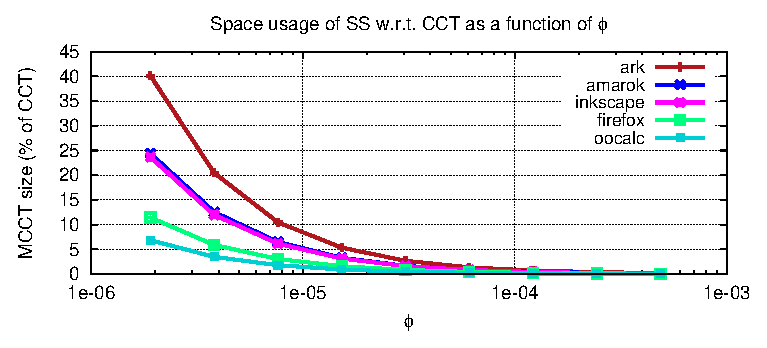
\includegraphics[width=0.75\textwidth]{figures/hcct-space-by-phi/hcct-space-by-phi.eps}
\caption{\protect\label{fig:hcct-space-by-phi} Space usage as a function of the hotness threshold $\phi$..
}
\end{center}
\end{figure}
\fi

\ifdefined\noauthorea
\begin{figure}[!ht]
\begin{center}
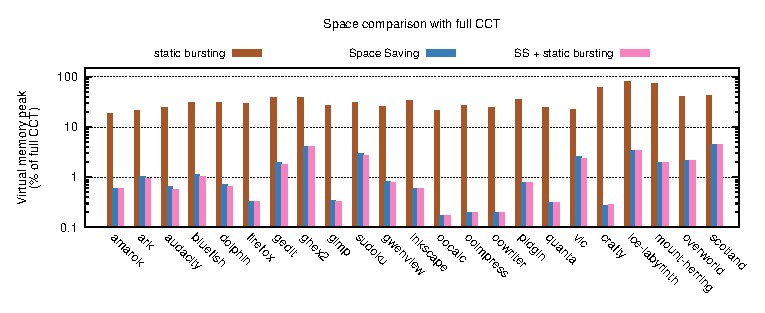
\includegraphics[width=\textwidth]{figures/hcct-space/hcct-space.eps}
\caption{\protect\label{fig:hcct-space} Space analysis of static bursting (left), SS (center), and SS combined with static bursting (right) with sampling interval 2 msec and burst length 0.2 msec.

%Space analysis on several benchmarks of static bursting~\cite{Zhuang06} (left), SS (center), and SS combined with static bursting (right) with sampling interval 2 msec and burst length 0.2 msec.

}
\end{center}
\end{figure}
\fi

As a second experiment, we study the actual memory footprint of our profilers considering both SS and the combination of SS with static bursting. \myfigure\ref{fig:hcct-space} plots the peak memory usage of our profilers as a percentage of the full CCT. We recall that during the computation we store the minimal subtree MCCT of the CCT spanning all monitored contexts. This subtree is eventually pruned to obtain the $(\phi,\varepsilon)$-HCCT (\mysection\ref{ss:hcct-approach,ss:hcct-algorithms}). The peak memory usage is proportional to the number of MCCT nodes, which is typically much larger than the actual number of hot contexts obtained after pruning.

Quite surprisingly, static bursting also improves space usage. This depends on the fact that sampling reduces the variance of calling context frequencies: MCCT cold nodes that have a hot descendant are more likely to become hot when sampling is active, and monitoring these nodes reduces the total MCCT size. The histogram also shows that static bursting alone (i.e., without streaming) is not sufficient to substantially reduce space: in addition to hot contexts, a large fraction of cold contexts is also sampled and included in the CCT. We also observed that the larger the applications, the larger the space reduction of our approach over bursting alone.

Since the average node degree is a small constant, cold HCCT nodes are typically a fraction of the total number of nodes, as shown in \myfigure\ref{fig:hcct-false-positives} for $\phi=10^{-4}$\ifauthorea{}{ (page \pageref{fig:hcct-false-positives})}. In our experiments we observed that this fraction strongly depends on the  hotness threshold $\phi$, and in particular decreases with $\phi$: cold nodes that have a hot descendant are indeed more likely to become hot when $\phi$ is smaller.

\subsection{Time Overhead}

We now discuss the time overhead of our approach, both alone and in combination with static bursting. We compare to native execution, to the widely-used call-graph profiler \gprof~\cite{Graham82}, and to the canonical CCT construction. To assess the instrumentation overhead, we also compare to {\em empty} instrumentation (i.e., when no analysis is performed).

\ifdefined\noauthorea
\begin{figure}[!ht]
\begin{center}
\begin{tabular}{cc}
\hspace{-6mm}
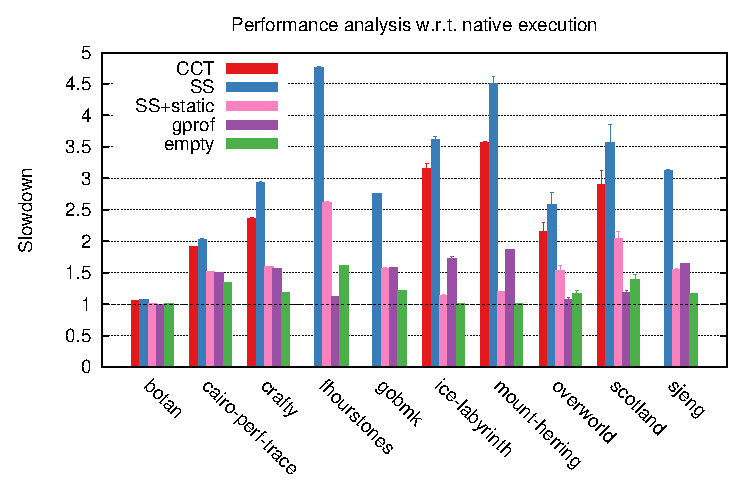
\includegraphics[width=0.49\textwidth]{figures/hcct-slowdown/hcct-slowdown-native.eps} &
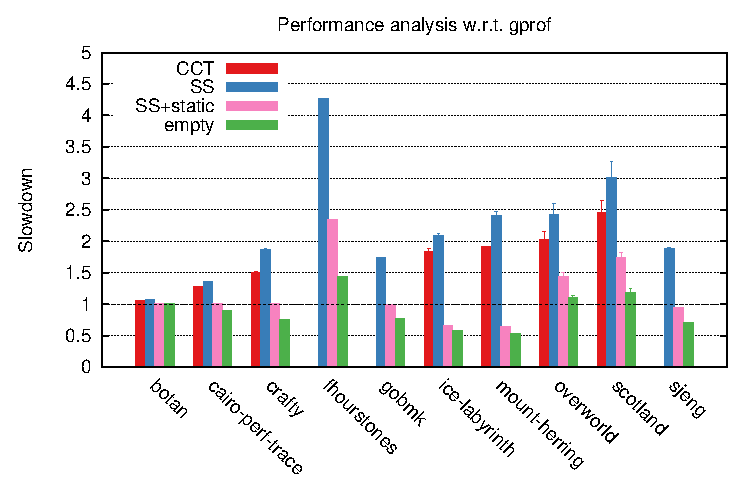
\includegraphics[width=0.49\textwidth]{figures/hcct-slowdown/hcct-slowdown-gprof.eps}\\
(a) & (b)
\end{tabular}
\caption{\protect\label{fig:hcct-slowdown} Runtime analysis for CCT and $(\phi,\varepsilon)$-HCCT construction compared to (a) native executions and (b) executions under \gprof. The {\em empty} bars measure the cost of instrumenting function calls and returns. SS with stating bursting has been executed with sampling interval 20 msec and burst length 2 msec.
}
\end{center}
\end{figure}
\fi

\myfigure\ref{fig:hcct-slowdown}(a) shows the overheads of the different profilers normalized against the performance of a native execution. The average slowdown for the CCT construction is $2.45\times$, with a peak of $3.56\times$ for {\tt mount-herring}. Note that data for benchmarks {\tt fhourstones}, {\tt gobmk} and {\tt sjeng} are not reported for the CCT profiler as it ran out of memory. We observe that the construction of the $(\phi,\varepsilon)$-HCCT incurs an average slowdown of $2.9\times$ ($3.09\times$ considering also OOM benchmarks) and is $16.28\%$ slower than the CCT profiler, with a peak of $26.08\%$ for {\tt mount-herring}. Given the previously discussed memory usage reduction, this represents an interesting space-time trade-off.

The integration with static bursting reduces the average overhead of our approach to $1.58\times$ for the whole set of benchmarks, which is not far from the $1.21\times$ slowdown introduced by the {\tt gcc} instrumentation itself. We observe a peak of $2.62\times$ on the benchmark {\tt fhourstones}: we believe this is due to the particular structure of its source code, which contains very frequently invoked tiny functions that could be replaced with macros.

In \myfigure\ref{fig:hcct-slowdown}(b) we have normalized the runtime overheads against an execution under \gprof. The combination of our approach with static bursting is very effective, as it is on average $18\%$ ($5.16\%$ if we exclude {\tt fhourstones}) slower than \gprof. On 5 out of 10 benchmarks, the two tools achieve nearly-identical slowdowns. We observe $2.34\times$, $1.44\times$ and $1.74\times$ slowdowns on {\tt fhourstones}, {\tt overworld}, and {\tt scotland}, respectively. Notice that for all these benchmarks the cost of the instrumentation inserted by \gcc\ is already greater than the slowdown introduced by \gprof. On the other hand, we observe appreciable speedups on {\tt ice-labyrinth} and {\tt mount-herring}, for which SS combined with static bursting is $1.51\times$ and $1.55\times$ faster than \gprof, respectively.

\subsection{Accuracy}
% !TEX root = thesis.tex

%\section{{\em k-}iteration Path Profiling}
\section{Multi-iteration Path Profiling}
\label{ss:kblpp-eval}

In this section, we discuss and evaluate an implementation, which we call \kblpp, of our approach to multi-iteration path profiling in the Jikes Research Virtual Machine (RVM)~\cite{Alpern00}. Our code is publicly available in the Jikes RVM Research Archive\footnote{\url{http://sourceforge.net/p/jikesrvm/research-archive/41/}.} and has been endorsed by the OOPSLA 2013 Artifact Evaluation Committee. The goal of our experimental study is to assess the performance of our profiler compared to previous approaches and to study properties of path profiles that span multiple iterations for several representative benchmarks. The results indicate that our technique can profile paths that extend across many loop iterations in a time comparable with acyclic path profiling on a large variety of industrial-strength benchmarks.

\subsection{Implementation}
\label{ss:kblpp-implementation}

\paragraph*{Adaptive Compilation.}  Jikes RVM is a high-performance {\em meta-circular} virtual machine: unlike most other JVMs, it is written in Java. Jikes RVM does not include an interpreter: all bytecode must be first translated into native machine code. The unit of compilation is the method, and methods are compiled lazily by a fast non-optimizing compiler -- the so-called {\em baseline} compiler -- when they are first invoked by the program. As execution continues, the Adaptive Optimization System monitors program execution to detect program hot spots and selectively recompiles them with three increasing levels of optimization. This approach is typical of modern production JVMs, which rely on some variant of selective optimizing compilation to target the subset of the hottest program methods where they are expected to yield the most benefits.

Recompilation is performed by the {\em optimizing} compiler, that generates higher-quality code but at a significantly larger cost than the baseline compiler. Since Jikes RVM quickly recompiles frequently executed methods, we implemented \kblpp in the optimizing compiler only.

\paragraph*{Adding Instrumentation.} As discussed in \mysection\ref{ss:kblpp-approach}, the Ball-Larus tracing technique requires instrumenting CFG edges so that when an edge is traversed, the probe value is incremented by a quantity computed by the path numbering algorithm on the DAG obtained by transforming back edges in the CFG.

\kblpp\ adds instrumentation to hot methods in three passes:
\begin{enumerate}[itemsep=0pt]
 \item building the DAG representation;
 \item assigning values to edges;
 \item adding instrumentation to edges.
\end{enumerate}

\noindent \kblpp\ adopts the {\em smart path numbering} algorithm proposed by Bond and McKinley~\cite{Bond05b} to improve performance by placing instrumentation on cold edges. In particular, line 6 of the canonical Ball-Larus path numbering algorithm shown in \myalgorithm\ref{alg:kblpp-bl-numbering} \ifauthorea{}{(page \pageref{alg:kblpp-bl-numbering})} is modified such that outgoing edges are picked in decreasing order of execution frequency. For each basic block edges are sorted using existing edge profiling information collected by the baseline compiler: we can thus assign zero to the hottest hedge, so that \kblpp\ will not place any instrumentation on it.
%in this way we can assign zero to the hottest edge, thus allowing us to assign zero to the hottest edge so that \kblpp\ does not place any instrumentation on it.

During compilation, Jikes RVM introduces {\em yield points}, which are program points where the running thread determines whether it should yield to another thread. Since JVMs need to gain control of threads quickly, compilers insert yield points in method prologues, loop headers, and method epilogues. We modified the optimizing compiler to also store the path profiling probe on loop headers and method epilogues. Ending paths at loop headers rather than back edges causes a path that traverse a header to be split into two paths: this difference from canonical Ball-Larus path profiling is minor because it only affects the first path through a loop~\cite{Bond05}.

Note that optimizing compilers do not insert yield points in a method when either it does not contain branches (hence its profile is trivial) or it is marked as uninterruptible. The second case occurs in internal Jikes RVM methods only; the compiler occasionally inlines such a method into an application method, and this might result in a loss of information only when the execution reaches a loop header contained in the inlined method. However, according to \cite{Bond05}, this loss of information appears to be negligible.

\paragraph*{Path Profiling.} To make fair performance comparisons with state-of-the-art previous profilers, we built our code on top of the BLPP profiler developed by Bond~\cite{Bond05,PEP}, which provides an efficient implementation of the Ball-Larus acyclic-path profiling technique. The \ksf\ construction algorithm described in \mysection\ref{ss:kblp-algorithms} is implemented using a standard first-child, next-sibling representation for nodes. This representation is very space-efficient, as it requires only two pointers per node: one to its leftmost child and the other to its right nearest sibling. % - while experimental results show that the average degree of a node is usually low.

\ifdefined\noauthorea
\begin{figure}[!ht]
\begin{center}
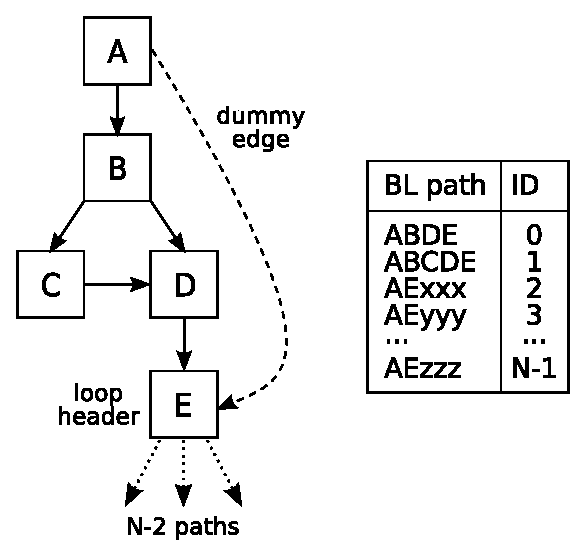
\includegraphics[width=0.4\textwidth]{figures/kblpp-example-fewer/kblpp-example-fewer.eps}
\caption{\protect\label{fig:kblpp-example-fewer} Routine with an initial branch before the first cycle.}
\end{center}
\end{figure}
\fi

\noindent Tree roots are stored and accessed through an efficient implementation\footnote{{\tt HashMapRVM} is a stripped-down implementation of the {\tt HashMap} data structure used by core parts of the Jikes RVM runtime and by Bond's BLPP path profiler.} of a hash map, using the pair represented by the Ball-Larus path ID and the unique identifier associated to the current routine (i.e., the compiled method ID) as key. Note that this map is typically smaller than a map required by a traditional BLPP profiler, since tree roots represent only a fraction of the distinct path IDs encountered during the execution. Consider, for instance, the example shown in \myfigure\ref{fig:kblpp-example-fewer}: this control flow graph has $N$ acylic paths after backedges have been removed. Since cyclic paths are truncated on loop headers, only path IDs $0$ and $1$ can appear after the special marker $*$ in the stream, thus leading to the creation of an entry in the hash map. Additional entries might be created when a new tree is added to the \ksf\ (line 10 of the streaming algorithm shown in \myalgorithm\ref{alg:kblpp-ksf-algorithm}\ifauthorea{}{ on page \pageref{alg:kblpp-ksf-algorithm}}); however, experimental results show that the number of tree roots is usually small, while $N$ increases with the complexity (i.e., number of branches and loops) of the routine.

\subsection{Experimental Setup}

In this section we illustrate the details of our experimental methodology, focusing on benchmarks, performance and topological metrics, and compared profiling techniques.

\subsubsection*{Benchmarks}

We evaluated \kblpp\ against a variety of prominent benchmarks drawn from three suites. The \dacapo\ suite~\cite{Blackburn06} consists of a set of open source, real-world applications with non-trivial memory loads. We use the superset of all benchmarks from \dacapo\ releases 2006-10-MR2 and 9.12 that can run successfully in Jikes RVM, using the largest available workload for each benchmark. In particular, {\tt avrora}, {\tt jython}, {\tt luindex}, {\tt sunflow}, and {\tt xalan} are taken from the 9.12 release, while {\tt chart}, {\tt eclipse}, and {\tt hsqldb} are from the 2006-10-MR2 release.

The \specjvm\ suite~\cite{SpecJVM2008} focuses on the performance of the hardware processor and memory subsystem when executing common general purpose application computations. Benchmarks from the suite that can run successfully\footnote{Due to limitations of the GNU classpath, only a small number of them are supported.} on Jikes RVM include: {\tt compiler.compiler}, {\tt compress}, {\tt mpegaudio}, and {\tt scimark.\{montecarlo, sor.large, sparse.large\}}.

Finally, we chose two memory-intensive benchmarks ({\tt heapsort} and {\tt md}) from the \javagrande\ $2.0$ suite~\cite{Bull99} to further evaluate the performance of \kblpp.

\subsubsection*{Metrics}
We considered a variety of metrics, including wall-clock time, number of operations per second performed by the profiled program, number of hash table operations, data structure size (e.g., number of hash table items for \blpp\ and number of \ksf\ nodes for \kblpp), and statistics such as average node degree of the \ksf\ and the \kipf\ and average depth of \kipf\ leaves. To interpret our results, we also ``profiled our profiler'' by collecting hardware performance counters with {\tt perf}~\cite{perf}, including L1 and L2 cache miss rate, branch mispredictions, and cycles per instruction (CPI).

\subsubsection*{Compared Codes}
In our experiments, we analyzed the native (uninstrumented) version of each benchmark and its instrumented counterparts, comparing \kblpp\ for different values of $k$ (2, 3, 4, 6, 8, 11, 16) with the \blpp\ profiler developed by Bond~\cite{PEP} for Ball-Larus acyclic-path profiling. We upgraded the original tool by Bond to take advantage of native threading support introduced in later Jikes RVM releases; the code is structured as in \myfigure\ref{fig:kblpp-approach}\ifauthorea{}{ (page \pageref{fig:kblpp-approach})}, except that it does not produce any intermediate stream, but it directly performs {\tt count[r]++}.

\subsubsection*{Platform}
In our experiments we used a 2.53GHz Intel Core2 Duo T9400 with 128KB of L1 data cache, 6MB of L2 cache, and 4 GB of main memory DDR3 1066, running Ubuntu 12.10, Linux Kernel 3.5.0, 32 bit. We ran all of the benchmarks on Jikes RVM 3.1.3 (default {\tt production} build) using a single core and a maximum heap size equal to half of the amount of physical memory. For each benchmark/profiler combination, we performed 10 trials, each preceded by a warm-up execution, and computed the arithmetic mean. We collected performance measurements with negligible background activity. We report confidence intervals stated at 95\% confidence level.

\subsection{Time Overhead}
\label{ss:eval-kblpp-time}

In \myfigure\ref{fig:kblpp-slowdown} we report for each benchmark the profiling overhead of \kblpp\ relative to \blpp. The chart shows that for 12 out of 16 benchmarks the overhead decreases for increasing values of $k$, providing up to almost 45\% improvements over \blpp. This is explained by the fact that hash table accesses are performed by {\tt process\_bl\_path\_id} every $k-1$ items read from the input stream between two consecutive routine entry events (lines 8 and 10 in \myalgorithm\ref{alg:kblpp-ksf-algorithm}\ifauthorea{)}{on page \pageref{alg:kblpp-ksf-algorithm})}. As a consequence, the number of hash table operations for each routine call is $O(1+N/(k-1))$, where $N$ is the total length of the path taken during the invocation.

\ifdefined\noauthorea
\begin{figure}[!ht]
\begin{center}
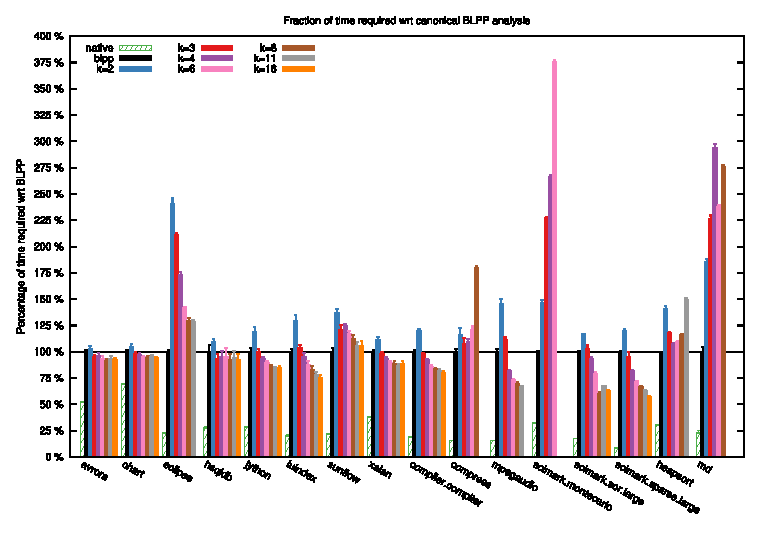
\includegraphics[width=\textwidth]{figures/kblpp-slowdown/kblpp-slowdown.eps}
\caption{\protect\label{fig:kblpp-slowdown} Performance of \kblpp\ relative to \blpp.
}
\end{center}
\end{figure}
\fi

In \myfigure\ref{fig:kblpp-hash} we report the measured number of hash table accesses for our experiments, which decreases as predicted on all benchmarks with intense loop iteration activity. Notice that not only does \kblpp\ perform fewer hash table operations, but since only a subset of BL path IDs are inserted, the table is also smaller, thus yielding further performance improvements. For codes such as {\tt avrora} and {\tt hsqldb}, which perform on average a small number of iterations, increasing $k$ beyond this number does not yield any benefit.

\ifdefined\noauthorea
\begin{figure}[!ht]
\begin{center}
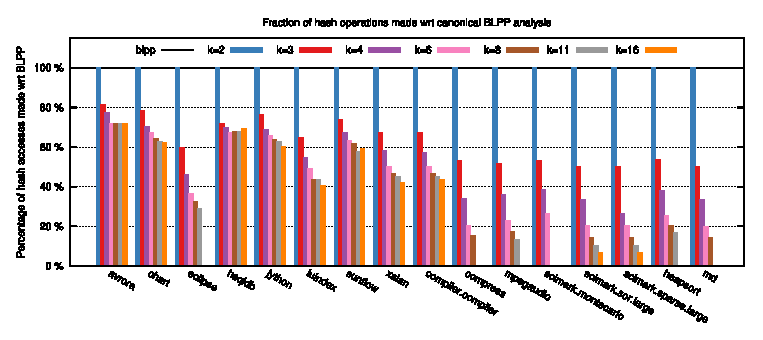
\includegraphics[width=\textwidth]{figures/kblpp-hash/kblpp-hash.eps}
\caption{\protect\label{fig:kblpp-hash} Number of hash table operations performed by \kblpp\ relative to \blpp.
}
\end{center}
\end{figure}
\fi

On {\tt eclipse}, \kblpp\ gets faster as $k$ increases, but differently from all other benchmarks in this class, it remains slower than \blpp\ by at least 25\%. The reason is that, due to structural properties of the benchmark, the average number of node scans at lines 13 and 21 of {\tt process\_bl\_path\_id} is rather high (58.8 for $k=2$ down to 10.3 for $k=16$). In contrast, the average degree of internal nodes of the \ksf\ is small (2.6 for $k=2$ decreasing to 1.3 for $k=16$), hence there is intense activity on nodes with a high number of siblings. No other benchmark exhibited this extreme behavior. We expect that a more efficient implementation of {\tt process\_bl\_path\_id}, e.g., by adaptively moving hot children to the front of the list, could reduce the scanning overhead for this kind of worst-case benchmarks as well.

\noindent Benchmarks {\tt compress}, {\tt scimark.montecarlo}, {\tt heapsort}, and {\tt md} made an exception to the general trend we observed, with performance overhead increasing, rather than decreasing, with $k$. To explain this behavior, we collected and analyzed several hardware performance counters and noticed that on these benchmarks our \kblpp\ implementation suffers from increased CPI for higher values of $k$.

\ifdefined\noauthorea
\begin{figure}[!ht]
\begin{center}
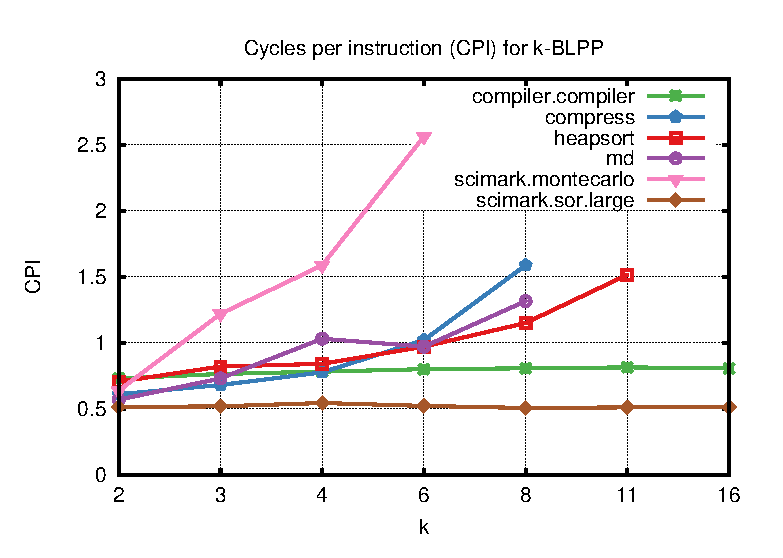
\includegraphics[width=0.49\textwidth]{figures/kblpp-cpi/kblpp-cpi.eps}
\caption{\protect\label{fig:kblpp-cpi} Hardware performance counters for \kblpp: cycles per instruction (CPI).
}
\end{center}
\end{figure}
\fi

\vspace{2em}
\noindent\myfigure\ref{fig:kblpp-cpi} shows this phenomenon, comparing the four outliers with other benchmarks in our suite. By analyzing L1 and L2 cache miss rates, reported in \myfigure\ref{fig:kblpp-cache} (a) and \myfigure\ref{fig:kblpp-cache} (b), we noticed that performance degrades due to poor memory access locality. We believe this to be an issue of our current implementation of \kblpp, in which we did not make any effort aimed at improving cache efficiency in accessing the \ksf, rather than a limitation of the general approach we propose. Indeed, as nodes may be unpredictably scattered in memory due to the linked structure of the forest, pathological situations may arise where node scanning incurs several cache misses.

\ifdefined\noauthorea
\begin{figure}[!ht]
\begin{center}
\begin{tabular}{cc}
\hspace{-6mm}
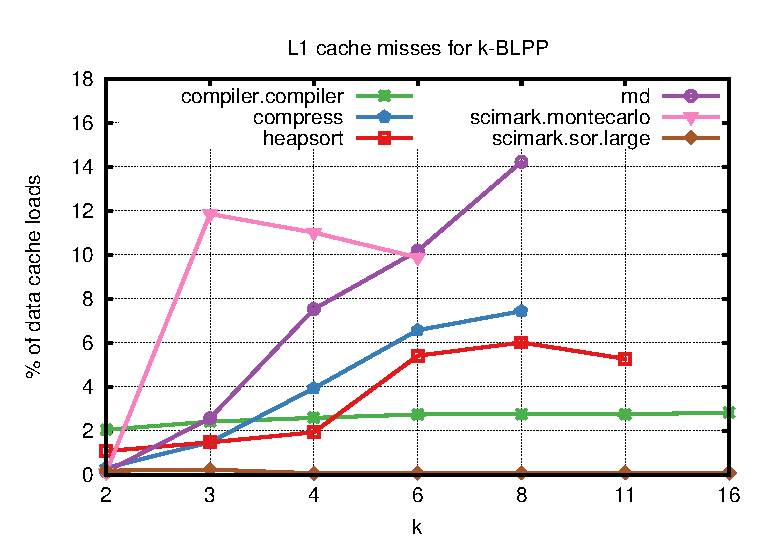
\includegraphics[width=0.49\textwidth]{figures/kblpp-cache/kblpp-cache-L1.eps} &
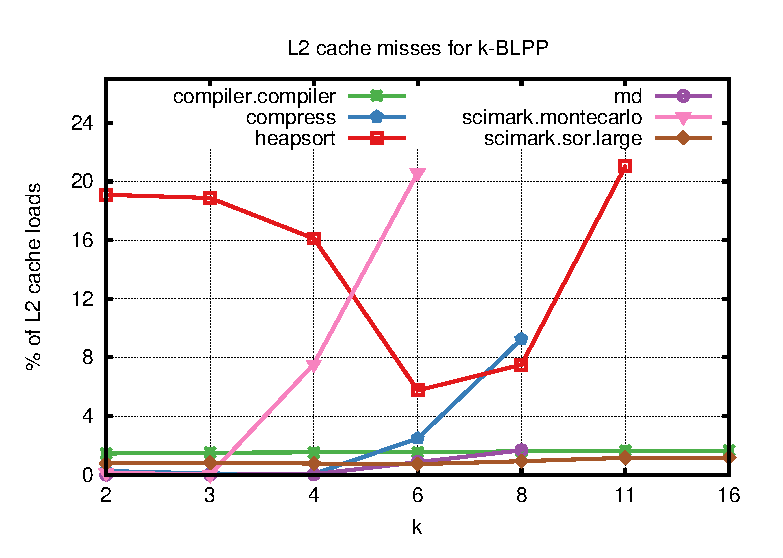
\includegraphics[width=0.49\textwidth]{figures/kblpp-cache/kblpp-cache-L2.eps}\\
(a) & (b)
\end{tabular}
\caption{\protect\label{fig:kblpp-cache} Hardware performance counters for \kblpp: (a) L1 and (b) L2 cache miss rates.}
\end{center}
\end{figure}
\fi

%\noindent Notice that since we never delete either entries from the hash table or nodes from the \ksf, our implementation does not place any additional burden on the garbage collector. The profiler causes memory release operations only when a thread terminates, dumping all of its data structures at once.

\noindent Notice that since we never delete either entries from the hash table or nodes from the \ksf, the only load we place on the garbage collector comes from allocating new nodes when needed. In fact, the profiler causes memory release operations only when a thread terminates, dumping all of its data structures at once.

\subsection{Memory Usage and Structural Properties}
\myfigure\ref{fig:kblpp-space} compares the space requirements of \blpp\ and \kblpp\ for different values of $k$. The chart reports the total number of items stored in the hash table by \blpp\ and the number of nodes in the \ksf.

\ifdefined\noauthorea
\begin{figure}[!ht]
\begin{center}
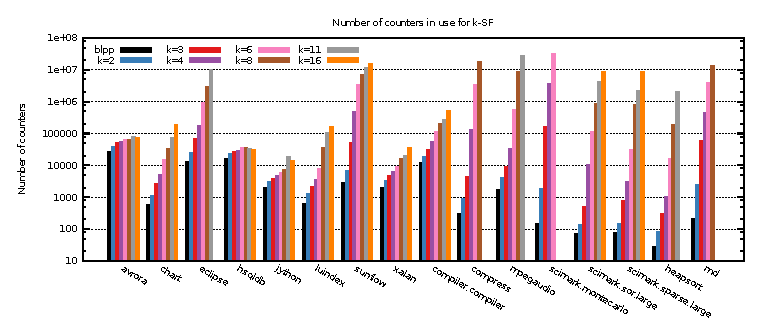
\includegraphics[width=\textwidth]{figures/kblpp-space/kblpp-space.eps}
\caption{\protect\label{fig:kblpp-space} Space requirements: number of hash table entries in \blpp\ and number of nodes in the \ksf.

}
\end{center}
\end{figure}
\fi

\vspace{-1em}

\ifdefined\noauthorea
\begin{figure}[!ht]
\begin{center}
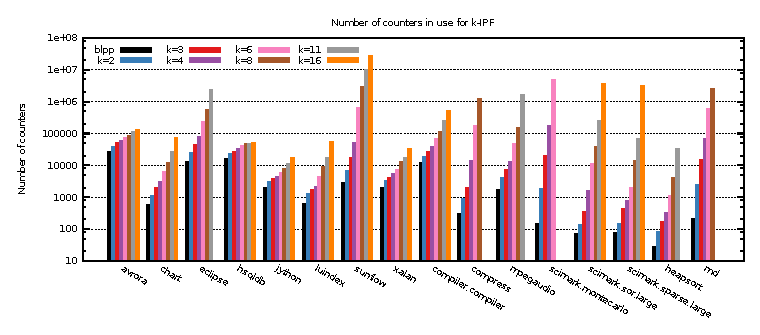
\includegraphics[width=\textwidth]{figures/kblpp-space-kipf/kblpp-space-kipf.eps}
\caption{\protect\label{fig:kblpp-space-kipf} Number of paths profiled by \blpp\ and \kblpp.

}
\end{center}
\end{figure}
\fi

\noindent Since both \blpp\ and \kblpp\ exhaustively encode exact counters for all distinct taken paths of bounded length, space depends on intrinsic structural properties of the benchmark. Programs with intense loop iteration activity are characterized by substantially higher space requirements by \kblpp, which collects profiles containing up to several millions of paths. Notice that on some benchmarks we ran out of memory for large values of $k$, hence some bars in the charts we report in this section are missing. In \myfigure\ref{fig:kblpp-space-kipf} we report the number of nodes in the \kipf, which corresponds to the number of paths profiled by \kblpp. Notice that since a path may be represented more than once in the \ksf, the \kipf\ represents a more compact version of the \ksf.

\noindent As a final experiment, we measured structural properties of the \kipf\ such as average degree of internal nodes (\myfigure\ref{fig:kblpp-kipf-degree}) and the average leaf depth (\myfigure\ref{fig:kblpp-kipf-leaves}). Our tests reveal that the average node degree generally decreases with $k$, showing that similar patterns tend to appear frequently across different iterations. Some benchmarks, however, such as {\tt sunflow} and {\tt heapsort} exhibit a larger variety of path ramifications, witnessed by increasing node degrees at deeper levels of the \kipf. The average leaf depth allows us to characterize the loop iteration activity of different benchmarks. Notice that for some benchmarks, such as {\tt avrora} and {\tt hsqldb}, most cycles consist of a small number of iterations: hence, by increasing $k$ beyond this number, \kblpp\ does not collect any additional useful information.

\ifdefined\noauthorea
\begin{figure}[!ht]
\begin{center}
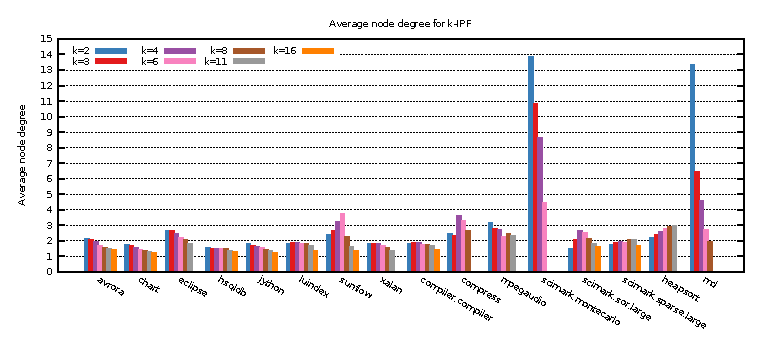
\includegraphics[width=\textwidth]{figures/kblpp-kipf-degree/kblpp-kipf-degree.eps}
\caption{\protect\label{fig:kblpp-kipf-degree} Average degree of \kipf\ internal nodes.

}
\end{center}
\end{figure}
\fi

\vspace{-1em}

\ifdefined\noauthorea
\begin{figure}[!ht]
\begin{center}
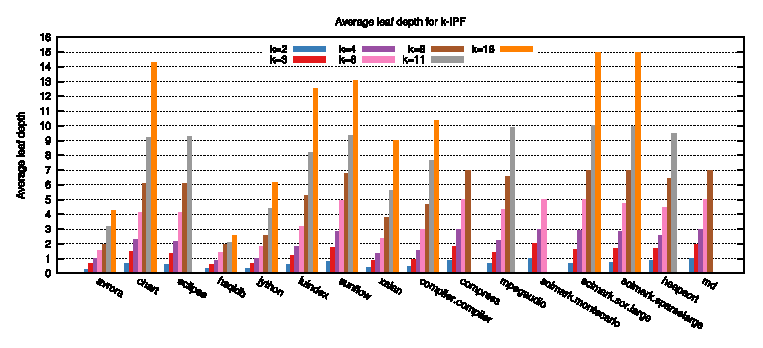
\includegraphics[width=\textwidth]{figures/kblpp-kipf-leaves/kblpp-kipf-leaves.eps}
\caption{\protect\label{fig:kblpp-kipf-leaves} Average depth of \kipf\ leaves.

}
\end{center}
\end{figure}
\fi

\subsection{Discussion}
Compared to previous approaches that enumerate $k$-iteration paths explicitly using numerical identifiers (\mysection\ref{ss:kblpp-related}), our prefix forest-based solution resorts to the original Ball-Larus encoding algorithm and maintains an intermediate data structure, the \ksf, that can be updated in constant time regardless of the value of $k$. Our technique can be faster than the original Ball-Larus algorithm on large programs, as it performs fewer operations on possibly smaller hash tables; for the same reason, its run-time overhead typically decreases for increasing values of $k$. We believe that our implementation is amenable to interesting enhancements, for instance by devising pruning heuristics in order to scale to larger values of $k$, or by having a separate thread construct the \ksf\ from the stream of BL path IDs emitted by an instrumented program's thread.

% !TEX root = thesis.tex

\section{OSR in LLVM}
\label{se:eval-osrkit}

In this section we present an experimental study of \osrkit. In particular, we aim at addressing the following questions:

\begin{description}[labelindent=1em ,labelsep*=1em,leftmargin=3.5em,itemsep=3pt,parsep=3pt]
\item[Q1] How much does a never-firing OSR point impact code quality? What kind of slowdown should we expect?
\item[Q2] What is the run-time overhead of an OSR transition, for instance to a clone of the running function?
\item[Q3] What is the overhead of \osrkit\ for inserting OSR points and creating a stub or a continuation function?
\end{description}

\noindent Experimental results suggest that inserting an OSR point is unlikely to degrade the quality of generated code, and that the time spent in IR manipulation is likely to be dominated by compilation costs. For an optimizer, the choice whether to insert an OSR point into a function merely depends on the trade-off between the expected benefits in terms of execution time and the overhead from generating the new code version: compared to this task, the cost of OSR-related operations is negligible.

\subsection{Experimental Setup}

\subsubsection*{Benchmarks}
We address questions Q1-Q3 by analyzing the performance of \osrkit\ on a selection of the \shootout\ benchmarks, also known as the Computer Language Benchmarks Game~\cite{shootout}, running in \tinyvm. In particular, we focus on single-threaded benchmarks that do not rely on external libraries to perform their core computations. Benchmarks and their description are reported in \mytable\ref{tab:osr-shootout}; four of them ({\tt b-trees}, {\tt mbrot}, {\tt n-body} and {\tt sp-norm}) are evaluated against two workloads of different size.

We generate the IR modules for our experiments with \clang\ starting from the C version of the \shootout\ suite. To cover scenarios where OSR machinery is inserted in programs with different optimization levels, we consider two versions: 1) {\em unoptimized}, where the only LLVM optimization we perform is \memtoreg\ to promote stack references to registers and construct the SSA form; 2) {\em optimized}, where we apply {\tt opt} {\tt -O1} to the unoptimized version.

\begin{table}[!hb]
\begin{center}
\begin{small}
    \begin{tabular}{ |c|c| }
        \hline
        Benchmark & Description \\
        \hline
        \hline
        b-trees & Adaptation of a GC bench for binary trees \\
        \hline
        fannkuch & Fannkuch benchmark on permutations \\
        \hline
        fasta & Generation of DNA sequences \\
        \hline
        fasta-redux & Generation of DNA sequences (with lookup table) \\
        \hline
        mbrot & Mandelbrot set generation \\
        \hline
        n-body & N-body simulation of Jovian planets \\
        \hline
        rev-comp & Reverse-complement of DNA sequences \\
        \hline
        sp-norm & Eigenvalue calculation with power method \\
        \hline
    \end{tabular}
\end{small}
\end{center}
\caption{\label{tab:osr-shootout} Description of the \shootout\ benchmarks.}
\end{table}

\subsubsection*{Environment}
\tinyvm\ supports interactive invocations of functions and it can compile LLVM IR either generated at run time or loaded from disk. The main design goal behind \tinyvm\ is the creation of an interactive environment for IR manipulation and JIT-compilation of functions: for instance, it allows the user to insert OSR points in loaded functions, run optimization passes on them or display their CFGs, repeatedly invoke a function for a specified amount of times and so on.

\tinyvm\ supports dynamic library loading and linking, and comes with a helper component for MCJIT that simplifies tasks such as handling multiple IR modules, symbol resolution in the presence of multiple versions of a function, and tracking native code and other machine-level generated object such as Stackmaps (\mysection\ref{ss:osrkit-implementation}). \tinyvm\ is thus an ideal playground to exercise our OSR technique.

\subsubsection*{Platform}
We performed our experiments on an octa-core 2.3Ghz Intel Xeon E5-4610 v2 with 256+256KB of L1 cache, 2MB of L2 cache, 16MB of shared L3 cache, and 128 GB of DDR3 main memory, running Debian Wheezy 7, Linux kernel 3.2.0, LLVM 3.6.2 (Release build, compiled using gcc 4.7.2), 64 bit. For each benchmark we analyze CPU time performing 10 trials preceded by an initial warm-up iteration; reported confidence intervals are stated at 95\% confidence level.

\subsection{Impact on Code Quality}

In order to measure how much a never-firing OSR point might impact code quality (Q1), we analyzed the source-code structure of each benchmark and profiled its run-time behavior to identify performance-critical sections for OSR point insertion. The distinction between open and resolved OSR points is nearly irrelevant in this context: we choose to focus on open OSR points, passing {\tt null} as the {\tt val} argument for the stub (see \mysection\ref{ss:osrkit-implementation}).

For iterative benchmarks, we insert an OSR point in the body of their hottest loops. We classify a loop as hottest when its body is executed for a very high cumulative number of iterations (e.g., from millions up to billions) and it either calls the method with the highest {\em self} time in the program, or it performs the most computational-intensive operations for the program in its own body.

\ifdefined\noauthorea
\begin{figure}[t]
\begin{center}
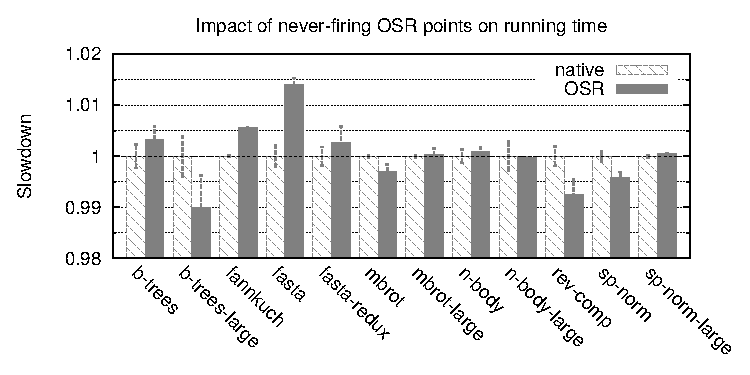
\includegraphics[width=0.65\textwidth]{figures/osr-code-quality-base/osr-code-quality-base.eps}
\caption{\protect\label{fig:osr-code-quality-base} Q1: Impact on running time of never-firing OSR points inserted inside hot code portions (unoptimized code).


}
\end{center}
\end{figure}
\fi

\ifdefined\noauthorea
\begin{figure}[t]
\begin{center}
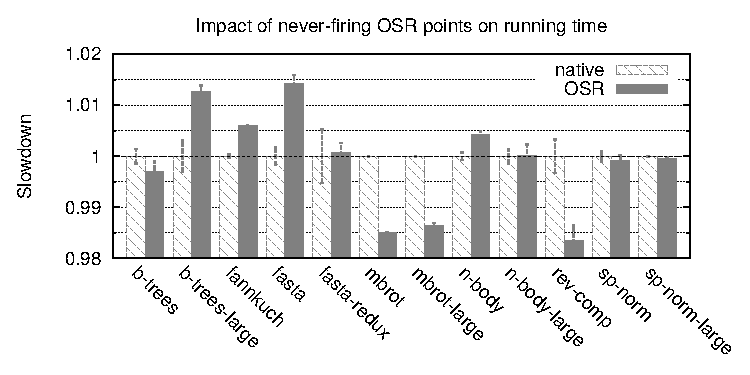
\includegraphics[width=0.65\textwidth]{figures/osr-code-quality-O1/osr-code-quality-O1.eps}
\caption{\protect\label{fig:osr-code-quality-O1} Q1: Impact on running time of never-firing OSR points inserted inside hot code portions (optimized code).



}
\end{center}
\end{figure}
\fi

These loops are natural candidates for OSR point insertion: for instance, Jikes RVM inserts yield points on backward branches to trigger operations such as method recompilation through OSR and thread preemption for garbage collection. In the \shootout\ benchmarks, the number of such loops is typically 1 (2 for {\tt spectral-norm}).

For recursive benchmarks, we insert an OSR point in the body of the method that accounts for the largest {\em self} execution time in the program. Such an OSR point might be useful to trigger recompilation of the code at a higher degree of optimization, enabling for instance multiple levels of inlining for non-tail-recursive functions. The only analyzed benchmark showing a recursive pattern is {\tt b-trees}.

Results for the unoptimized and optimized versions of the benchmarks are reported in \myfigure\ref{fig:osr-code-quality-base} and \myfigure\ref{fig:osr-code-quality-O1}, respectively. For both scenarios we observe that the overhead is very small, i.e., less than $1\%$ for most benchmarks and less than $2\%$ in the worst case. For some benchmarks, code might run slightly faster after OSR point insertion due to instruction cache effects.
%We analyzed the code produced by the x86-64 back-end: the OSR machinery is lowered into three native instructions that load a counter in a register, compare it against a constant value and jump to the OSR block accordingly.
The number of times the OSR condition is checked for each benchmark is
%the same as in the experiments
reported in \mytable\ref{tab:osr-sameFun}.

\subsection{Overhead of OSR Transitions}

\mytable\ref{tab:osr-sameFun} reports estimates of the average cost of performing an OSR transition to a clone of the running function (Q2). For each benchmark we compute the time difference between the scenarios in which an always-firing and a never-firing resolved OSR point is inserted in the code, respectively; we then normalize this difference against the number of fired OSR transitions.

\begin{table}[ht]
\begin{center}
\begin{small}
    \begin{tabular}{ |c|C{1.33cm}|C{1.00cm}|C{1.15cm}|C{1.00cm}|C{1.15cm}| }
        \cline{3-6}
        \multicolumn{2}{c|}{} & \multicolumn{2}{c|}{{\em Unoptimized code}} & \multicolumn{2}{c|}{{\em Optimized code}} \\
        \hline
        Benchmark & Fired OSRs (M) & Live values & Avg time (ns) & Live values & Avg time (ns) \\
        \hline
        \hline
        b-trees & 605 & 2 & 1.731 & 3 & 0.974 \\
        \hline
        b-trees-large & 2\,690 & 2 & 1.749 & 3 & 1.423 \\
        \hline
        fannkuch & 399 & 0 & 1.793 & 0 & 0.621 \\
        \hline
        fasta & 400 & 2 & 2.335 & 2 & 2.699 \\
        \hline
        fasta-redux & 400 & 4 & 2.306 & 4 & 2.269 \\
        \hline
        mbrot & 256 & 15 & 5.016 & 15 & 3.628 \\
        \hline
        mbrot-large & 1\,024 & 15 & 5.268 & 15 & 4.637 \\
        \hline
        n-body & 50 & 3 & 2.952 & 3 & 6.929 \\
        \hline
        n-body-large & 500 & 3 & 2.953 & 3 & 6.953 \\
        \hline
        rev-comp & 6 & 8 & -10.158 & 8 & 8.267 \\
        \hline
        sp-norm & 1\,210 & 2 & 0.772 & 2 & -0.030 \\
        \hline
        sp-norm-large & 19\,360 & 2 & 0.778 & 2 & -0.003 \\
        \hline
    \end{tabular}
\end{small}
\end{center}
\caption{\label{tab:osr-sameFun}Cost of OSR transitions to the same function. For each benchmark we report the number of fired OSR transitions (rounded to millions), the number of live values passed at the OSR point, and the average time for a transition.
}
\end{table}

\noindent Hot code portions for OSR point insertion have been identified as in the Q1 experiments for code quality. Depending on the characteristics of the hot loop, we either transform its body into a separate function and instrument its entrypoint, or, when the loop calls a method with a high self time, we insert an OSR point at the beginning of that method.

Normalized differences reported in the table represent a reasonable estimate of the average cost of firing an OSR transition, which consists in moving live values to stack locations or registers to match the calling convention and then invoking the OSR continuation function.
%, which in other words is the cost of performing a function call passing the live variables as arguments.
Reported numbers are in the order of nanoseconds, and might be negative due to instruction cache effects. We remark that for this experiment slicing the loop body is preferable to inserting an OSR point in it, as the continuation function should fire an OSR itself at the very next loop iteration and so on, possibly leading to an undesired stack growth.

\subsection{OSR Machinery Generation}

We now discuss the overhead of the \osrkit\ library for inserting OSR machinery in the IR of a function (Q3). \mytable\ref{tab:osr-instrTime} reports for each benchmark the number of IR instructions in the instrumented function and the time spent in the IR manipulation. Locations for OSR points are chosen as in the Q1 experiments, and the target function is a clone of the source function.

\begin{table}[ht]
\begin{center}
\begin{small}
    \begin{tabular}{ |c|c|c|c|c|c|c| }
        \cline{3-7}
        \multicolumn{2}{l|}{} & \multicolumn{2}{c|}{{\em Open OSR {\tiny$(\mu s)$}}} & \multicolumn{3}{c|}{{\em Resolved OSR  {\tiny$(\mu s)$}}} \\
        \cline{3-7}
        \multicolumn{2}{l|}{} & Insert & Gen. & Insert & \multicolumn{2}{|c|}{Generate \fosrto} \\
        \cline{1-2} \cline{6-7}
        Benchmark & \textbar IR\textbar & point & stub & point & Total & Avg/inst \\
        \hline
        \hline
        b-trees & 13 & 15.40 & 28.32 & 14.31 & 76.13 & 5.86 \\
        \hline
        fannkuch & 50 & 14.16 & 18.66 & 12.84 & 208.03 & 4.16 \\
        \hline
        fasta & 38 & 12.93 & 27.07 & 13.01 & 250.39 & 6.59 \\
        \hline
        fasta-redux & 55 & 13.79 & 23.44 & 9.32 & 258.36 & 4.70 \\
        \hline
        mbrot & 77 & 15.96 & 27.39 & 15.30 & 384.61 & 4.99 \\
        \hline
        n-body & 19 & 14.31 & 19.73 & 11.58 & 88.73 & 4.67  \\
        \hline
        rev-comp & 145 & 16.31 & 39.99 & 13.90 & 810.84 & 5.59 \\
        \hline
        sp-norm & 28 & 15.31 & 27.50 & 12.41 & 154.54 & 5.52 \\
        \hline
    \end{tabular}
\end{small}
\end{center}
\caption{\label{tab:osr-instrTime} Q3: OSR machinery insertion in optimized code. Time measurements are expressed in microseconds. Results for unoptimized code are very similar and thus not reported.}
\end{table}

\noindent For open OSR points, we report the time spent in inserting the OSR point in the function and in generating the stub; both operations do not depend on the size of the function. For resolved OSR points, we report the time spent in inserting the OSR point and in generating the \fosrto\ function.

Not surprisingly, constructing a continuation function takes longer than the other operations (i.e., up to 1 ms vs. 20-40 us), as it involves cloning and manipulating the body of the target function and thus depends on its size: \mytable\ref{tab:osr-instrTime} hence comes with an additional column in which time is normalized against the number of IR instructions in the target function.

%On our benchmarks, the overall cost of IR manipulation is in the order of hundreds of microseconds, and is thus very likely to be dominated by the cost of just-in-time compilation.

\subsection{Discussion}
Our results suggest that the LLVM MCJIT compiler is able to generate efficient native code for the OSR machinery inserted in performance-critical code sections. The overall cost of IR manipulation for inserting an OSR point insertion and generating a continuation function is in the order of hundreds of microseconds on our benchmarks, and will likely be dominated by the time spent in just-in-time compilation. We present an example of effective optimization enabled by \osrkit\ in \mysection\ref{se:CS-matlab}. 

%Hence, for a front-end the choice of whether to insert an OSR point for optimization essentially depends on the performance gains from recompilation.

%%%%%%%%%%%%%%%%%%%%%%%%%%%%%%%%%%%%%%%%%%%

%\section{On-Stack Replacement \`{a} la Carte}
%\section{OSR Mapping Generation}
\section{Building OSR Compensation Code}
\label{se:eval-OSR-alC}

In this section we evaluate our implementation in LLVM of the techniques for automatic OSR mapping construction described in \mysection\ref{se:osr-a-la-carte}. In particular, we investigate whether in the presence of a number of common compiler optimizations, the algorithm \buildcomp\ can offer an extensive ``menu'' of possible program points where OSR can safely occur, generating the possibly required compensation code in an automated fashion. Our experiments suggest that bidirectional OSR transitions can be supported almost everywhere in this setting.

\subsection{Experimental Setup}
\label{ss:bc-exp-setup}

\subsubsection*{Benchmarks and Environment}
We implemented our technique in \tinyvm, introducing a number of features to:
\begin{itemize}
 \item clone a function $f_{base}$ and apply a sequence of OSR-aware optimization passes, thus generating an optimized version $f_{opt}$;
 \item construct and compose OSR mappings for the applied transformations;
 \item for each feasible OSR point in $f_{base}$/$f_{opt}$, invoke \osrkit\ to materialize the compensation code $\chi$ produced by \reconstruct\ into a sequence of IR instructions for the OSR entry block of $f'_{opt}$/$f'_{base}$ (\mysection\ref{ss:osr-llvm-approach}).
\end{itemize}

\noindent We instrumented a number of standard LLVM optimization passes, including {\em aggressive dead code elimination} (ADCE), {\em constant propagation} (CP), {\em common subexpression elimination} (CSE), {\em loop-invariant code motion} (LICM), {\em sparse conditional constant propagation} (SCCP), and {\em code sinking} (Sink). We also instrumented a number of utility passes required by LICM, such as {\em natural loop canonicalization} (LC) and {\em LCSSA-form construction} (LCSSA). Optimizations performed by the back-end (e.g., instruction scheduling, register allocation, peephole optimizations) do not require instrumentation as we operate at the IR level.

We evaluated our technique on the \speccpu~\cite{Henning06} and the \phoronixpts~\cite{Phoronix} benchmarking suites, reporting data for a subset of their C/C++ benchmarks. We profiled each benchmark to identify the hottest method and generated the IR for it using \clang\ with no optimization enabled other than \memtoreg. Starting from this version of the IR, which we will refer to as {\em base}, we generated an {\em opt} version by applying all our instrumented LLVM optimizations.

The list of benchmarks and transformations that are effective on their hottest method is reported in \mytable\ref{tab:OSR-alC-bench-desc}. Numbers reported in \mytable\ref{tab:OSR-alC-bench-IR} for the IR manipulations performed by the transformations suggest that, while the {\em opt} version is typically shorter than its {\em base} counterpart, it might have a larger number of $\phi$-nodes (most of them are inserted during the LCSSA-form construction). We observed that SCCP was able to eliminate a large number of unreachable blocks for \mytt{ffmpeg}, while for the remaining benchmarks the majority of instruction deletions are performed by CSE, which replaces all of the uses of these instructions in the rest of the code with uses of equivalent available instructions.

\begin{table}[t]
\begin{center}
\begin{small}
\begin{tabular}{ |c|c|c|c|c|c|c|c|c|c| }
        \cline{3-10}
        \multicolumn{2}{l|}{} & \multicolumn{6}{c|}{Optimizations} & \multicolumn{2}{c|}{Utilities} \\
        \hline
        Suite & Benchmark & \em{ADCE} & \em{CP} & \em{CSE} & \em{SCCP} & \em{LICM} & \em{Sink} & \em{LC} & \em{LCSSA} \\
        \hline
        \hline
        \multirow{7}{*}{SPEC} & bzip2 & & & \checkmark & & \checkmark & \checkmark & & \checkmark \\
        \cline{2-10}
        & h264ref & \checkmark & & \checkmark & & \checkmark & \checkmark & \checkmark & \checkmark \\
        \cline{2-10}
        & hmmer & & & \checkmark & & \checkmark & \checkmark & & \checkmark \\
        \cline{2-10}
        & namd & \checkmark & \checkmark & \checkmark & \checkmark & \checkmark & \checkmark & & \checkmark \\
        \cline{2-10}
        & perlbench & \checkmark & & \checkmark & & \checkmark & \checkmark & \checkmark & \checkmark \\
        \cline{2-10}
        & sjeng & & & \checkmark & \checkmark & \checkmark & \checkmark & & \checkmark \\
        \cline{2-10}
        & soplex & & & \checkmark & \checkmark & \checkmark & \checkmark & & \\
        \hline
        \hline
        \multirow{5}{*}{PTS} & bullet & & \checkmark & \checkmark & & \checkmark & \checkmark & & \checkmark \\
        \cline{2-10}
        & dcraw & & & \checkmark & & \checkmark & \checkmark & \checkmark & \checkmark \\
        \cline{2-10}
        & ffmpeg & \checkmark & \checkmark & \checkmark & & \checkmark & \checkmark & \checkmark & \checkmark \\
        \cline{2-10}
        & fhourstones & & \checkmark & \checkmark & & \checkmark & & \checkmark & \checkmark \\
        \cline{2-10}
        & vp8 & & & \checkmark & & \checkmark & \checkmark & & \checkmark \\
        \hline
    \end{tabular}
\end{small}
%\end{adjustbox}
\end{center}
\caption{\label{tab:OSR-alC-bench-desc} Optimizations and utility passes effective on the hottest function of each benchmark. Optimization passes have been applied in the same order (left-to-right) as they appear in the table. Utility passes {\em LC} and {\em LCSSA} are pre-requisites of {\em LICM}.}
\end{table}

\begin{table}[!t]
\begin{center}
\begin{small}
\begin{tabularx}{0.9\textwidth}{|c|X|c|c|c|c|}
\cline{3-6}
\multicolumn{2}{l|}{} & \multicolumn{2}{c|}{base} & \multicolumn{2}{c|}{opt} \\
\hline
Benchmark & Function & $|\pi|$ & $|\phi|$ & $|\pi|$ & $|\phi|$ \\
\hline
\hline
bzip2 & mainSort & 657 & 32 & 596 & 44 \\
\hline
h264ref & SetupFastFullPelSearch & 671 & 28 & 576 & 36 \\
\hline
hmmer & P7Viterbi & 568 & 6 & 383 & 8 \\
\hline
namd & ComputeNonbondedUtil::calc\_pair\_ energy\_fullelect & 1737 & 159 & 1636 & 224 \\
\hline
perlbench & S\_regmatch & 5574 & 305 & 5001 & 355 \\
\hline
sjeng & std\_eval & 1940 & 93 & 1540 & 105 \\
\hline
soplex & SPxSteepPR::entered4X & 195 & 2 & 154 & 2 \\
\hline
bullet & btGjkPairDetector::getClosestPoints NonVirtual & 587 & 24 & 553 & 42 \\
\hline
dcraw & vng\_interpolate & 590 & 37 & 545 & 49 \\
\hline
ffmpeg & decode\_cabac\_residual\_internal & 618 & 34 & 462 & 40 \\
\hline
fhourstones & ab & 288 & 29 & 284 & 39 \\
\hline
vp8 & vp8\_full\_search\_sadx8 & 334 & 41 & 299 & 60 \\
\hline
\end{tabularx}

\vspace{6mm}

\begin{tabular}{|c|c|c|c|c|c|c|c|}
\hline
Benchmark & Added & Deleted & Hoisted & Sunk & $RAUW_I$ & $RAUW_C$ & $RAUW_A$ \\
\hline
\hline
bzip2 & 16 & 77 & 12 & 3 & 71 & 0 & 2 \\
\hline
h264ref & 9 & 105 & 4 & 21 & 102 & 0 & 0 \\
\hline
hmmer & 2 & 187 & 13 & 1 & 187 & 0 & 0 \\
\hline
namd & 68 & 169 & 36 & 73 & 145 & 17 & 0 \\
\hline
perlbench & 86 & 667 & 96 & 28 & 627 & 0 & 0 \\
\hline
sjeng & 13 & 413 & 20 & 34 & 412 & 1 & 0 \\
\hline
soplex & 0 & 41 & 2 & 4 & 41 & 0 & 0 \\
\hline
bullet & 26 & 60 & 37 & 3 & 51 & 1 & 0 \\
\hline
dcraw & 13 & 58 & 25 & 6 & 58 & 0 & 0 \\
\hline
ffmpeg & 11 & 168 & 9 & 17 & 52 & 51 & 0 \\
\hline
fhourstones & 14 & 20 & 3 & 0 & 14 & 2 & 0 \\
\hline
vp8 & 19 & 54 & 17 & 34 & 54 & 0 & 0 \\
\hline
\end{tabular}
\end{small}
%\end{adjustbox}
\end{center}
\caption{\label{tab:OSR-alC-bench-IR} Details on the IR manipulations on the hottest function of each benchmark. For each function we report the number of instructions $|\pi|$ ($|\phi|$ of which represent $\phi$-nodes) for both the {\em base} and the {\em opt} version. We then report the number of primitive actions for code manipulations tracked across the applied transformations. $RAUW_{\{A,C,I\}}$ is used to indicate \RAUWfull\ actions performed for some {$N$} having Argument, Constant, or Instruction type in LLVM.
}
\end{table}

\subsubsection*{Platform}
We performed our experiments on a machine equipped with an Intel Core i7-3632QM processor, running Ubuntu 14.10, LLVM 3.6.2 (Release build), 64 bit.

\subsection{OSR to Optimized Version}

\myfigure\ref{fig:osr-BC-BtoO} shows the fraction of program points that are feasible for an OSR from {\em base} to {\em opt} depending on the version of \reconstruct\ being used (\mysection\ref{ss:BC-implementation}).

Locations that can fire an OSR with no need of a compensation code (i.e., $\chi=\langle\rangle$) account for a limited fraction of all the potential OSR points (less than $10\%$ for most benchmarks). This suggests that optimizations can significantly modify a program's live state across program locations.

\begin{figure}[!t]
\begin{center}
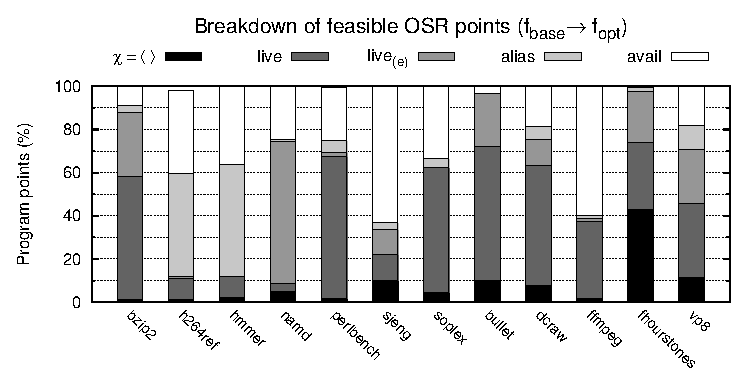
\includegraphics[width=0.8\textwidth]{figures/osr-BC-BtoO/osr-BC-BtoO.eps}
\caption{\protect\label{fig:osr-BC-BtoO} Fraction of program points that are OSR-feasible (from {\em base} to {\em opt}).

}
\end{center}
\end{figure}

We observe that the $live$ version of \reconstruct\ performs well on some benchmarks (e.g., \mytt{perlbench}, \mytt{bullet}, \mytt{dcraw}) and poorly on others (e.g., \mytt{h264ref}, \mytt{namd}). The enhancements introduced in the $live_{(e)}$ version are effective for some benchmarks (e.g., \mytt{namd}, \mytt{sjeng}), while aliasing information exploited in the $alias$ version increases the number of feasible OSR points for all benchmarks. For $9$ out of $12$ of them, it is possible in fact to build a compensation code using only live variables at the OSR source for more than $60\%$ of potential OSR points.

When in the $avail$ version \reconstruct\ is allowed to extend the liveness range of an ``available'' variable, the percentage of feasible OSR points grows to nearly $100\%$. We observed for \mytt{bullet} that a specific $\phi$-node needs to be reconstructed at nearly $20\%$ of feasible OSR points: this node takes as incoming values a number of $\phi$-nodes that in turn all yield the same value. While LLVM's built-in method for detecting trivially constant $\phi$-nodes does not cover this case, our recursive heuristic introduced in the $live_{(e)}$ version is able to identify the value and use it directly.

\begin{table}[!ht]
\begin{center}
\begin{small}
\begin{tabular}{ |c|c|c|c|c|c|c|c|c| }
\cline{2-9}
\multicolumn{1}{l|}{} & \multicolumn{2}{c|}{$|\chi|\leftarrow live_{(e)}$} & \multicolumn{2}{c|}{$|\chi|\leftarrow alias$} & \multicolumn{2}{c|}{$|\chi|\leftarrow avail$} & \multicolumn{2}{c|}{$|K_{avail}|$} \\
\hline
Benchmark & Avg & Max & Avg & Max & Avg & Max & Avg & Max \\
\hline
\hline
bzip2 & 4.29 & 14 & 4.3 & 14 & 4.73 & 13 & 3.6 & 8 \\
\hline
h264ref & 1.94 & 2 & 2.9 & 5 & 3.37 & 5 & 1.02 & 2 \\
\hline
hmmer & 3.3 & 5 & 16.11 & 23 & 16.63 & 24 & 4.02 & 7 \\
\hline
namd & 18.48 & 28 & 18.61 & 28 & 17.82 & 28 & 3.38 & 6 \\
\hline
perlbench & 46.29 & 57 & 46.12 & 57 & 45.82 & 57 & 1.24 & 12 \\
\hline
sjeng & 9.51 & 21 & 9.72 & 21 & 18.52 & 32 & 4.2 & 12 \\
\hline
soplex & 5.08 & 7 & 5.02 & 7 & 4.38 & 7 & 2.34 & 4 \\
\hline
bullet & 16.79 & 46 & 16.69 & 46 & 15.93 & 46 & 6.15 & 17 \\
\hline
dcraw & 7.72 & 15 & 7.6 & 15 & 7.32 & 15 & 1.97 & 7 \\
\hline
ffmpeg & 5.22 & 8 & 5.05 & 8 & 4.03 & 8 & 1.85 & 3 \\
\hline
fhourstones & 4.64 & 6 & 4.5 & 6 & 4.98 & 6 & 1.7 & 2 \\
\hline
vp8 & 9.6 & 16 & 10.51 & 16 & 10.13 & 17 & 2.35 & 6 \\
\hline
\hline
Avg & {\bf 11.07} & 18.75 & {\bf 12.26} & 20.50 & {\bf 12.81} & 21.50 & {\bf 2.82} & 7.17 \\
\hline
\end{tabular}
\end{small}
\end{center}
\caption{\label{tab:OSR-alC-prologue-BtoO} Average and peak size $|\chi|$ of the compensation code generated by the $live_{(e)}$, $alias$, and $avail$ versions of algorithm \reconstruct. $|K_{avail}|$ is the size of the set of variables that we should artificially keep alive in order to make program points represented by white bars in \myfigure\ref{fig:osr-BC-BtoO} feasible for an OSR from {\em base} to {\em opt}.}
\end{table}

In \mytable\ref{tab:OSR-alC-prologue-BtoO} we report the average and peak size of the compensation code $\chi$ generated by the $live_{(e)}$, $alias$, and $avail$ variants of \reconstruct\ across feasible OSR points. Figures for $live$ are not reported as they would not add much to the discussion. Note also that average values have been calculated for different sets of program points, although the set of a version includes the set of the previous version.

The assignment step of \reconstruct\ (line 9 in \myalgorithm\ref{alg:osr-reconstruct}, page \pageref{alg:osr-reconstruct}) generates an average number of instructions typically smaller than $20$, with the notable exception of \mytt{perlbench}. Observe that \mytt{perlbench}'s hottest function \mytt{S\_regmatch} is highly amenable to CSE: we found out that no less than $583$ out of its $667$ deleted instructions (thus about $10\%$ of the {\em base} function - see \mytable\ref{tab:OSR-alC-bench-IR}) are removed by this optimization, and we believe that local CSE would shrink the OSR entry block of the continuation function $f'$ as well. However, we would like to remark that the size of $\phi$ is unlikely to affect the performance of $f'$ for a hot method, as compensation code will be located at the beginning of the function and executed only once.

The last two columns of \mytable\ref{tab:OSR-alC-prologue-BtoO} report the average and peak number of variables that are not live at the source location, but for which the $avail$ version of \reconstruct\ would artificially extend liveness to support OSR at more program points (i.e., those represented by the white portions of the bars in \myfigure\ref{fig:osr-BC-BtoO}). We observe that the average number of values to spill on the stack is less than $3$ for $9$ out of $12$ benchmarks, with a maximum of $6.16$ for \mytt{bullet}. $avail$ by default will extend the liveness of an available value only if it is not possible to reconstruct it: we implemented this strategy using a simple backtracking algorithm.

\subsection{OSR to Base Version}

\begin{figure}[!b]
\begin{center}
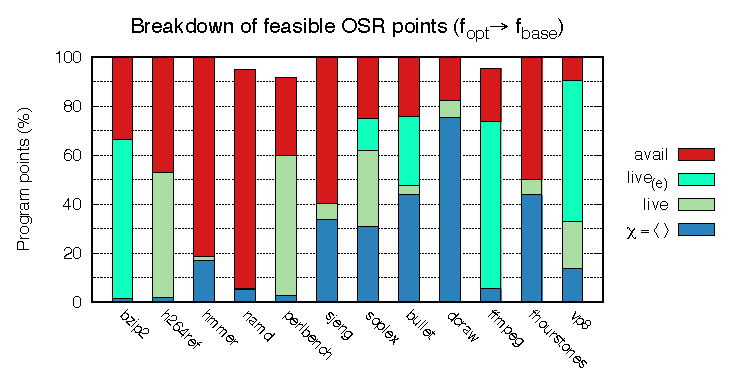
\includegraphics[width=0.8\textwidth]{figures/osr-BC-OtoB/osr-BC-OtoB.eps}
\caption{\protect\label{fig:osr-BC-OtoB} Fraction of program points that are OSR-feasible (from {\em opt} to {\em base}).


}
\end{center}
\end{figure}

\myfigure\ref{fig:osr-BC-OtoB} reports the fraction of OSR points eligible for {\em opt} to {\em base} deoptimization. We observe that the fraction of locations that can fire an OSR with an empty $\chi$ varies significantly from benchmark to benchmark, suggesting a dependence on the structure of the original program.

For $9$ out of $12$ benchmarks, compensation code can be built using only live variables for more than $50\%$ of potential OSR points.
%The assignment step of \reconstruct\ produces on average $2.3$ compensation instructions, with a peak of $5.74$ on \mytt{vp8}.
When the $avail$ version is used, the percentage of feasible OSR points is greater than $90\%$ on all benchmarks and nearly $100\%$ for $9$ out of $12$ of them.

\noindent Results for the $alias$ version of \reconstruct\ are not reported, as they do not improve those for $live_{(e)}$. Indeed, aliasing information is useful when a variable to set at the destination is aliased by multiple variables at the source, which we do not expect to happen in an optimized code.

\begin{table}[!ht]
\begin{center}
\begin{small}
\begin{tabular}{ |c|c|c|c|c|c|c| }
\cline{2-7}
\multicolumn{1}{l|}{} & \multicolumn{2}{c|}{$|\chi|\leftarrow live_{(e)}$} & \multicolumn{2}{c|}{$|\chi|\leftarrow avail$} & \multicolumn{2}{c|}{$|K_{avail}|$} \\
\hline
Benchmark & Avg & Max & Avg & Max & Avg & Max \\
\hline
\hline
bzip2 & 1.55 & 4 & 1.77 & 4 & 1.47 & 4 \\
\hline
h264ref & 4.46 & 9 & 2.82 & 9 & 1.45 & 7 \\
\hline
hmmer & 1 & 1 & 1 & 1 & 1.02 & 2 \\
\hline
namd & 1.5 & 2 & 5.93 & 15 & 4.74 & 18\\
\hline
perlbench & 4.09 & 12 & 4.22 & 12 & 1.37 & 11 \\
\hline
sjeng & 1.29 & 2 & 1.67 & 11 & 4.09 & 14 \\
\hline
soplex & 3.3 & 4 & 3.3 & 4 & 1.00 & 1 \\
\hline
bullet & 1 & 1 & 1.26 & 3 & 1.14 & 2 \\
\hline
dcraw & 1.68 & 2 & 3.84 & 6 & 4.06 & 8 \\
\hline
ffmpeg & 1.94 & 5 & 1.95 & 6 & 1.08 & 4 \\
\hline
fhourstones & 0 & 0 & 1.12 & 4 & 1.42 & 4 \\
\hline
vp8 & 5.74 & 13 & 5.51 & 13 & 1.18 & 5 \\
\hline
\hline
Avg & {\bf 2.30} & 4.58 & {\bf 2.87} & 7.33 & {\bf 2.00} & 6.67 \\
\hline
\end{tabular}
\end{small}
\end{center}
\caption{\label{tab:OSR-alC-prologue-OtoB} Average and peak size $|\chi|$ of the compensation code generated by the $live_{(e)}$ and $avail$ versions of algorithm \reconstruct. $|K_{avail}|$ is the size of the set of variables that we should artificially keep alive in order to make program points represented by white bars in \myfigure\ref{fig:osr-BC-OtoB} feasible for an OSR from {\em opt} to {\em base}.}
\end{table}

\noindent In \mytable\ref{tab:OSR-alC-prologue-OtoB} we report the average and peak size of the compensation code $\chi$ generated by the $live_{(e)}$ and $avail$ variants of \reconstruct\ across feasible OSR points, along with the average and peak number of available variables for which $avail$ artificially extends liveness to support OSR at program points represented by white bars in \myfigure\ref{fig:osr-BC-OtoB}. We observe that, compare to the {\em base}-to-{\em opt} case, the size of the compensation code is much smaller, suggesting that shorter portions of executions need to be reconstructed when ``OSR-ing'' to less optimized code.

Note that the $0$ values reported for \mytt{fhourstones} in the $live_{(e)}$ scenario do not imply that state compensation is not required. In fact, the algorithm detected that each variable $v$ to assign at the OSR landing pad for which no live counterpart was available at the source location, could be initialized with the value of either a (non-live) function argument or some live variable when $v$ is a constant $\phi$-node. In LLVM IR assignments of the form \mytt{x:=y} are not allowed, since all uses of \mytt{x} can simply be replaced with uses of \mytt{y}: for this reason, a \mytt{RAUW(x,y)} operation is performed on the body of the continuation function $f'$, where \mytt{y} is a live value transferred as argument for $f'$, and no instruction is added to the OSR entry block of $f'$.

\subsection{Discussion}
We have seen that common compiler transformations can significantly affect the live state of a program across its locations. The four versions of algorithm \reconstruct\ that we have implemented can generate compensation code automatically by recursively reassembling portions of the state for the target function.

OSR is enabled almost everywhere by the $avail$ version of the algorithm. Figures reported in \mytable\ref{tab:OSR-alC-prologue-BtoO,tab:OSR-alC-prologue-OtoB} suggest that the size of the set of virtual registers to preserve for an OSR from all supported locations is small: a compiler may thus spill available values that are not already located on the stack. When \reconstruct\ can resort only to live variables, it enables OSR at more than a half of the program locations. We observed that the reconstruction would often fail on an available value coming from a memory \load: we thus believe that the algorithm may significantly benefit from a simple alias analysis to identify safely repeatable \load\ instructions.

%For our benchmarks, we enable OSR from both unoptimized to optimized code and viceversa at more than a half of the program locations using only live variables at the source location, and almost anywhere when \reconstruct\ can access previously computed results that are still available.
\fi